% ------------------------------------------------------------------
\documentclass[12 pt]{article} % A4 paper set by geometry package below
\pagenumbering{arabic}
\setlength{\parindent}{10 mm}
\setlength{\parskip}{12 pt}

% Nimbus Sans font should be reasonably legible
\usepackage{helvet}
\renewcommand{\familydefault}{\sfdefault}
\usepackage[T1]{fontenc}  % Without this \textsterling produces $

% Section header spacing
\usepackage{titlesec}
\titlespacing\section{0pt}{12pt plus 4pt minus 2pt}{0pt plus 2pt minus 2pt}
\titlespacing\subsection{0pt}{12pt plus 4pt minus 2pt}{0pt plus 2pt minus 2pt}
\titlespacing\subsubsection{0pt}{12pt plus 4pt minus 2pt}{0pt plus 2pt minus 2pt}

\usepackage{amsmath}
\usepackage{amssymb}
\usepackage{graphicx}
\usepackage{verbatim}    % For comment
\usepackage[paper=a4paper, marginparwidth=0 cm, marginparsep=0 cm, top=2.5 cm, bottom=2.5 cm, left=3 cm, right=3 cm, includemp]{geometry}
\usepackage[pdftex, pdfstartview={FitH}, pdfnewwindow=true, colorlinks=true, citecolor=blue, filecolor=blue, linkcolor=blue, urlcolor=blue, pdfpagemode=UseNone]{hyperref}

% Put module code and last-modified date in footer
\usepackage{fancyhdr}
\pagestyle{fancy}
\fancyhf{}
\renewcommand{\headrulewidth}{0pt}
\cfoot{{\small \thisunit}\hfill \thepage\hfill {\small \moddate}}

% Hopefully address Canvas complaints about pdf tagging
%\usepackage[tagged]{accessibility}
\hypersetup {
  pdfauthor={David Schaich},
  pdftitle={Statistical Physics Tutorial Problem},
}
% ------------------------------------------------------------------



% ------------------------------------------------------------------
% Shortcuts
\newcommand{\be}{\ensuremath{\beta} }
\newcommand{\eps}{\ensuremath{\varepsilon} }
\newcommand{\om}{\ensuremath{\omega} }
\newcommand{\pderiv}[2]{\ensuremath{\frac{\partial #1}{\partial #2}} }
% ------------------------------------------------------------------



% ------------------------------------------------------------------
\begin{document}
\newcommand{\thisunit}{MATH327 Tutorial (Solid)}
\newcommand{\moddate}{Last modified 28 Mar.~2022}
\begin{center}
  {\Large \textbf{MATH327: Statistical Physics, Spring 2022}} \\[12 pt]
  {\Large \textbf{Tutorial problem \ --- \ Einstein solid}} \\[24 pt]
\end{center}

In Section~3.4 we computed the energy for $N$ distinguishable spins in a solid,
\begin{equation*}
  E = -NH\tanh(\be H)
\end{equation*}
for inverse temperature $\be = 1 / T$ and magnetic field strength $H$.
What is the corresponding heat capacity?
How does it compare to the experimental\footnote{Experimentally it is easier to measure the heat capacity at constant \textit{pressure}, $c_p$, rather than at constant volume, but the difference between $c_p$ and $c_v$ is negligible for our purposes here.} data points in the figure below (from Schroeder's \textit{Introduction to Thermal Physics})?

\begin{center}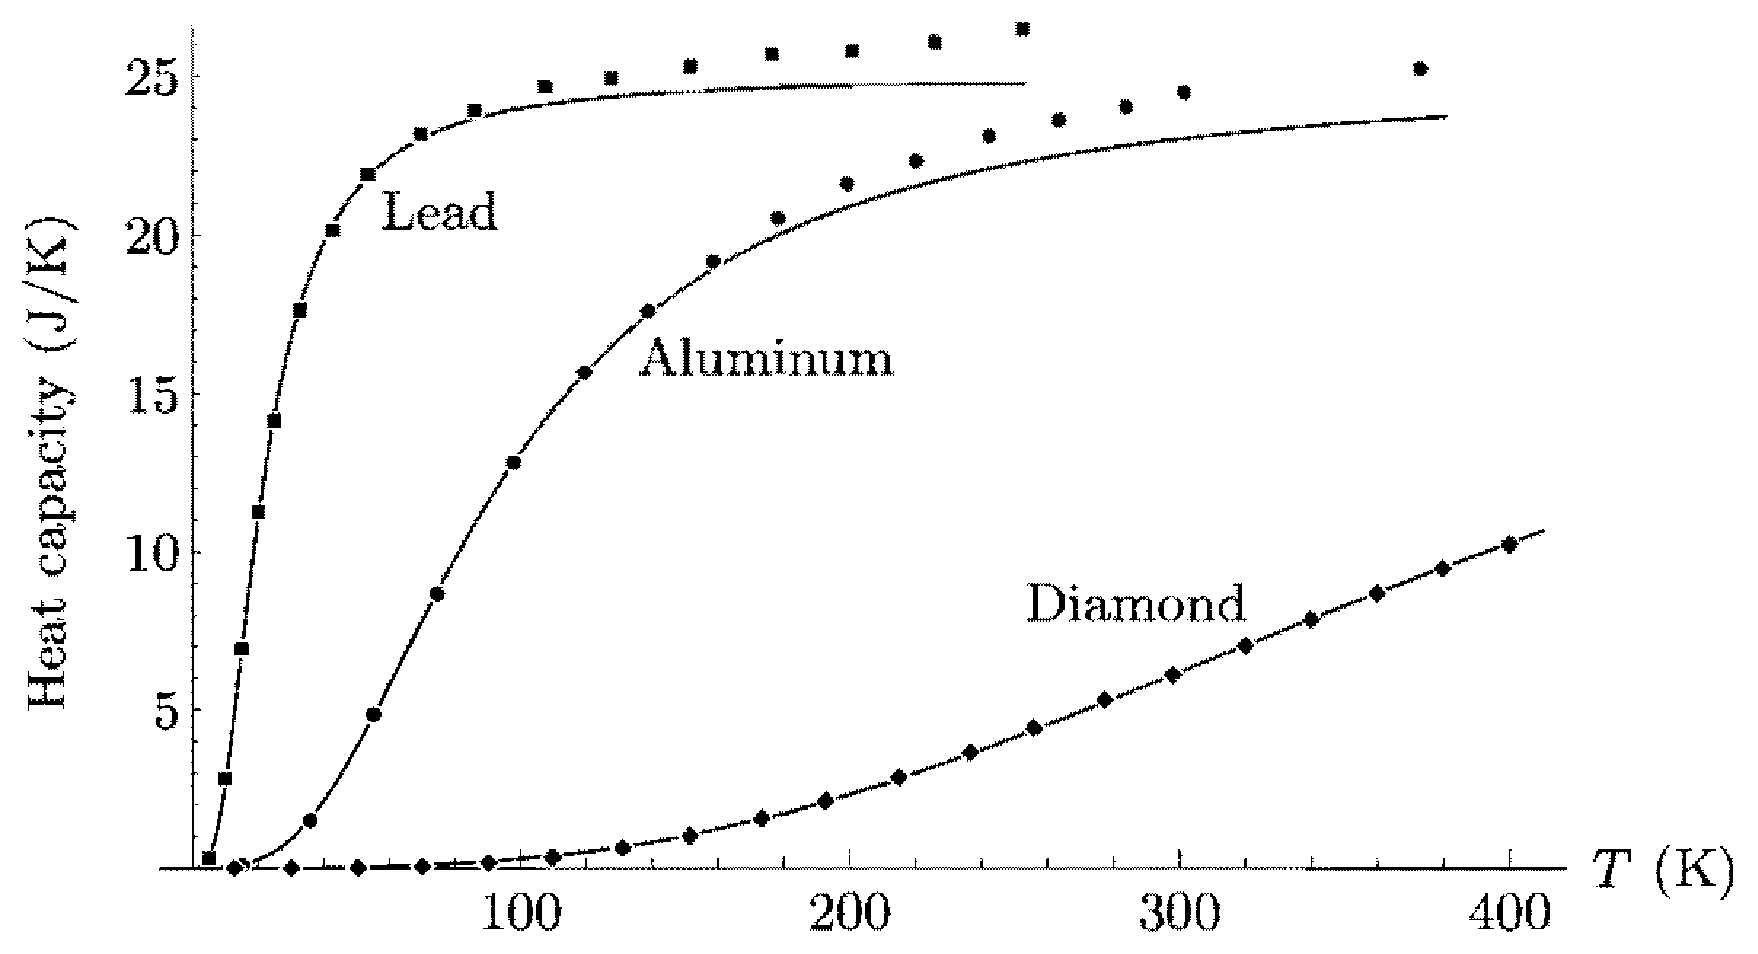
\includegraphics[width=0.8\textwidth]{figs/heat_cap.pdf}\end{center}

You should find poor agreement --- especially in the absence of an external field, $H = 0$!
This issue turns out to persist even for more realistic models of solids analyzed using classical approaches.
To address it, in 1907 Einstein developed a simple model of solids based on quantized energies, taking some inspiration from his 1905 proposal that quantized energies explain the \href{https://en.wikipedia.org/wiki/Photoelectric_effect}{photoelectric effect}.

The `Einstein solid' consists of many atoms whose positions are fixed to (distinguishable) locations in a regular lattice.
Interactions between neighbouring atoms are credited with pinning down each atom to its fixed location.
This is modeled by picturing neighbouring atoms connected by `oscillators', analogous to springs, which possess energy as a consequence of these interactions.
We define the Einstein solid by hypothesizing that the energy of each oscillator is quantized, $\eps_i = 0, \hbar \om$, $2\hbar \om$, $\cdots$, with the same characteristic angular frequency \om for all oscillators.
Although these oscillators model interactions between nearest-neighbour atoms, in this approach they are \textit{non-interacting} degrees of freedom that we can analyze using the statistical physics tools we have already developed.

As illustrated by the figure below, also from Schroeder's \textit{Introduction to Thermal Physics}, the number of oscillators depends both on the number of atoms and their layout.
In this two-dimensional square lattice, $N$ oscillators would correspond to $N / 2$ atoms in the solid.
In a three-dimensional cubic lattice, $N$ oscillators would correspond to $N / 3$ atoms. \\[-24 pt]
\begin{center}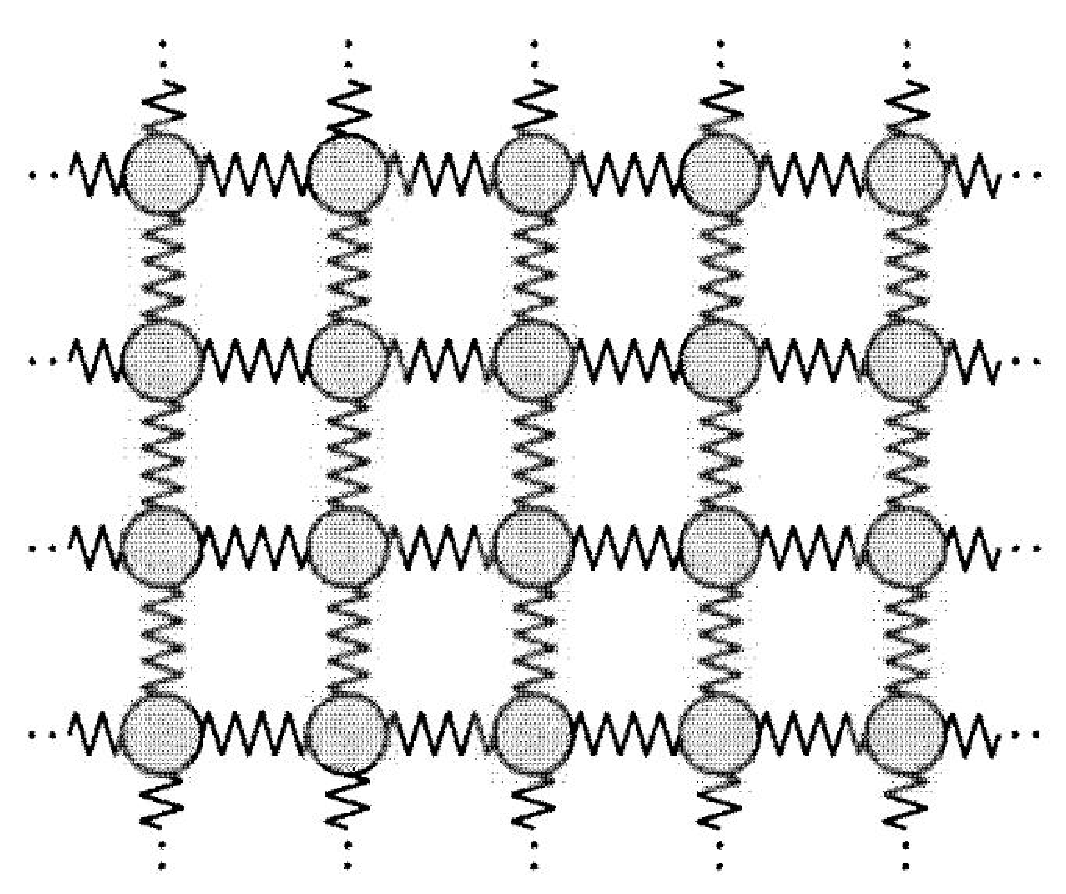
\includegraphics[width=0.5\textwidth]{figs/solid.pdf}\end{center}

Our goal is to compute the heat capacity for an Einstein solid.
Let's begin by working in terms of the micro-canonical ensemble, fixing the total energy
\begin{equation*}
  E = \sum_i \eps_i = \sum_i k_i\hbar\om \equiv K\hbar\om
\end{equation*}
where $K \equiv \sum_i k_i$ is the integer number of energy `units' available to be distributed among the $N$ oscillators.
Each different way of distributing these $K$ units of energy among the $N$ (distinguishable) oscillators defines a unique micro-state.

\begin{itemize}
  \item What is the total number of micro-states in terms of $N$ and $K$?
        Check your result for a minimal three-oscillator system when it has $K = 0$, $1$, $2$ or $3$ units of energy.

  \item Now consider $K \gg 1$ and $N \gg 1$, so that we can apply Stirling's formula and also approximate $N - 1 \approx N$ and $K - 1 \approx K$.
        What is the corresponding entropy?

  \item What is the temperature of the Einstein solid?
        Is it a `natural' system with $T > 0$?

  \item To find the heat capacity, we need to find the energy in terms of the temperature, then differentiate.
        What is the resulting heat capacity of the Einstein solid, in terms of $x \equiv \hbar \om / T$?
        How does it compare to the experimental data points we began by considering?
\end{itemize}

While the Einstein solid provides a significantly better description of the experimental data, room for improvement is still possible\dots

\end{document}
% ------------------------------------------------------------------
